%%%%%%%%%%%%%%%%%%%%%%% file template.tex %%%%%%%%%%%%%%%%%%%%%%%%%
%
% This is a general template file for the LaTeX package SVJour3
% for Springer journals.          Springer Heidelberg 2010/09/16
%
% Copy it to a new file with a new name and use it as the basis
% for your article. Delete % signs as needed.
%
% This template includes a few options for different layouts and
% content for various journals. Please consult a previous issue of
% your journal as needed.
%
%%%%%%%%%%%%%%%%%%%%%%%%%%%%%%%%%%%%%%%%%%%%%%%%%%%%%%%%%%%%%%%%%%%
%
% First comes an example EPS file -- just ignore it and
% proceed on the \documentclass line
% your LaTeX will extract the file if required
\begin{filecontents*}{example.eps}
%!PS-Adobe-3.0 EPSF-3.0
%%BoundingBox: 19 19 221 221
%%CreationDate: Mon Sep 29 1997
%%Creator: programmed by hand (JK)
%%EndComments
gsave
newpath
  20 20 moveto
  20 220 lineto
  220 220 lineto
  220 20 lineto
closepath
2 setlinewidth
gsave
  .4 setgray fill
grestore
stroke
grestore
\end{filecontents*}
%
\RequirePackage{fix-cm}
%
%\documentclass{svjour3}                     % onecolumn (standard format)
%\documentclass[smallcondensed]{svjour3}     % onecolumn (ditto)
\documentclass[twocolumn]{svjour3}       % onecolumn (second format)
%\documentclass[twocolumn]{svjour3}          % twocolumn
%
\smartqed  % flush right qed marks, e.g. at end of proof
%
\usepackage{graphicx}

%added by the author himself
\usepackage{color}
\usepackage[numbers]{natbib}



%
% \usepackage{mathptmx}      % use Times fonts if available on your TeX system
%
% insert here the call for the packages your document requires
%\usepackage{latexsym}
% etc.
%
% please place your own definitions here and don't use \def but
% \newcommand{}{}
%
% Insert the name of "your journal" with
% \journalname{myjournal}
%
\begin{document}

\title{AES and SNOW 3G are feasible choices for a 5G phone from energy perspective %\thanks{Grants or other notes
%about the article that should go on the front page should be
%placed here. General acknowledgments should be placed at the end of the article.}
}
%\subtitle{Do you have a subtitle?\\ If so, write it here}

%\titlerunning{Short form of title}        % if too long for running head

\author{Mohsin Khan         \and
        Valtteri Niemi %etc.
}

%\authorrunning{Short form of author list} % if too long for running head

\institute{Mohsin Khan \at
              University of Helsinki \\
              %Tel.: +123-45-678910\\
              %Fax: +123-45-678910\\
              \email{mohsin.khan@helsinki.fi}           %  \\
%             \emph{Present address:} of F. Author  %  if needed
           \and
           Valtteri Niemi \at
              University of Helsinki \\
              %Tel.: +123-45-678910\\
              %Fax: +123-45-678910\\
              \email{valtteri.niemi@helsinki.fi}  
}

\date{Received: date / Accepted: date}
% The correct dates will be entered by the editor


\maketitle

\begin{abstract}
The aspirations for a 5th generation (5G) mobile network are high. It has a vision of unprecedented data-rate and extremely pervasive connectivity. To cater such aspirations in a mobile phone, many existing efficiency aspects of a mobile phone need to be reviewed. We look into the matter of required energy to encrypt and decrypt the huge amount of traffic that will leave from and enter into a 5G enabled mobile phone. In this paper, we present an account of the power consumption details of the efficient hardware implementations of AES and SNOW 3G. We also present an account of the power consumption details of LTE protocol stack on some cutting edge hardware platforms. Based on the aforementioned two accounts, we argue that the energy requirement for the current encryption systems AES and SNOW 3G will not impact the battery-life of a 5G enabled mobile phone by any significant proportion.
\keywords{5G \and Cryptosystem \and ASIC}
% \PACS{PACS code1 \and PACS code2 \and more}
% \subclass{MSC code1 \and MSC code2 \and more}
\end{abstract}

\section{Introduction}
\label{intro} To facilitate our discussion, we need to know what are the data that will be encrypted and decrypted in a 5G phone. We also need to know where and how many times the encryption and decryption will take place across the protocol stack on the phone. But 5G is not yet a reality and we do not have exact answers to these questions. So, we assume things, that will be true for a 5G network and argue on the basis of those assumptions. We turn to the LTE network to make the assumptions. In an LTE phone, the data that leave and enter the phone can be broadly classified into three categories. The first one are the control signals in between the phone and the core network. The second one are the control signals in between the phone and the radio network. And the third one are the user data which the user sends and receives at the phone's application layer. Both of the first two categories are privacy and integrity protected. For the third category, only the privacy is protected. Also note that, from the volume point of view, the major share of data belong to the third category. Comparing to the the third category, the cryptographic computational need required for the data of first and second categories is negligible. The user data in an LTE phone is only once encrypted and decrypted across the protocol stack in PDCP layer. In an LTE phone this encryption is done by an application specific integrated circuit (ASIC).

For a 5G phone, we assume that the user data will remain as the major share of the total data leaving and entering the phone. The cryptographic computational need for the total volume of control signals will be negligible in comparison with that of the user data. The user data will only once be encrypted and decrypted somewhere across the protocol stack. From hardware point of view it will still be in an ASIC. In order to have a pessimistic estimation, we assume that integrity protection of user data will be introduced in 5G. Based on these assumptions, we will look into the cryptographic energy requirements and also the total energy requirements across the whole protocol stack of an LTE phone. Then we will scale up the data-rate from 100 Mbps to 1 Gbps and see how much extra pressure it puts on the battery of the phone in comparison with other energy hungry aspects of the phone like display and radio signalling.

The paper is organized by first giving a very short introduction to the architecture, the protocol stack and the cryptographic specifications of the LTE network in section \ref{sec:lte_specifications}. In section \ref{sec:throughput_and_energy_requirements_of_aes_snow3g}, we present the experimental results about the energy requirements of the two cryptosystems of interest, which are AES and SNOW 3G. In this section we also present the experimental result about the energy consumption across the whole protocol stack of the link layer. In section \ref{sec:overall_comparison} we present the energy consumption distribution of the whole phone among it's different functional modules and show that the energy needed for cryptographic computation is not a threat for the battery life of the phone. 


\section{LTE specifications}
\label{sec:lte_specifications}
An LTE network is comprised of broadly three components. The user equipment (UE), evolved radio network (E-UTRAN) known as radio network and evolved packet core (EPC) known as core network. The user equipment consists of a mobile equipment (ME) or a mobile phone for the context of this paper, and an universal integrated circuit card (UICC). The UICC hosts an application called subscriber identification module (SIM). In this paper when we refer to the user equipment, we mean it to be the mobile phone since the UICC does not have much functionality to consume a lot of energy.

\begin{figure}
% Use the relevant command to insert your figure file.
% For example, with the graphicx package use
  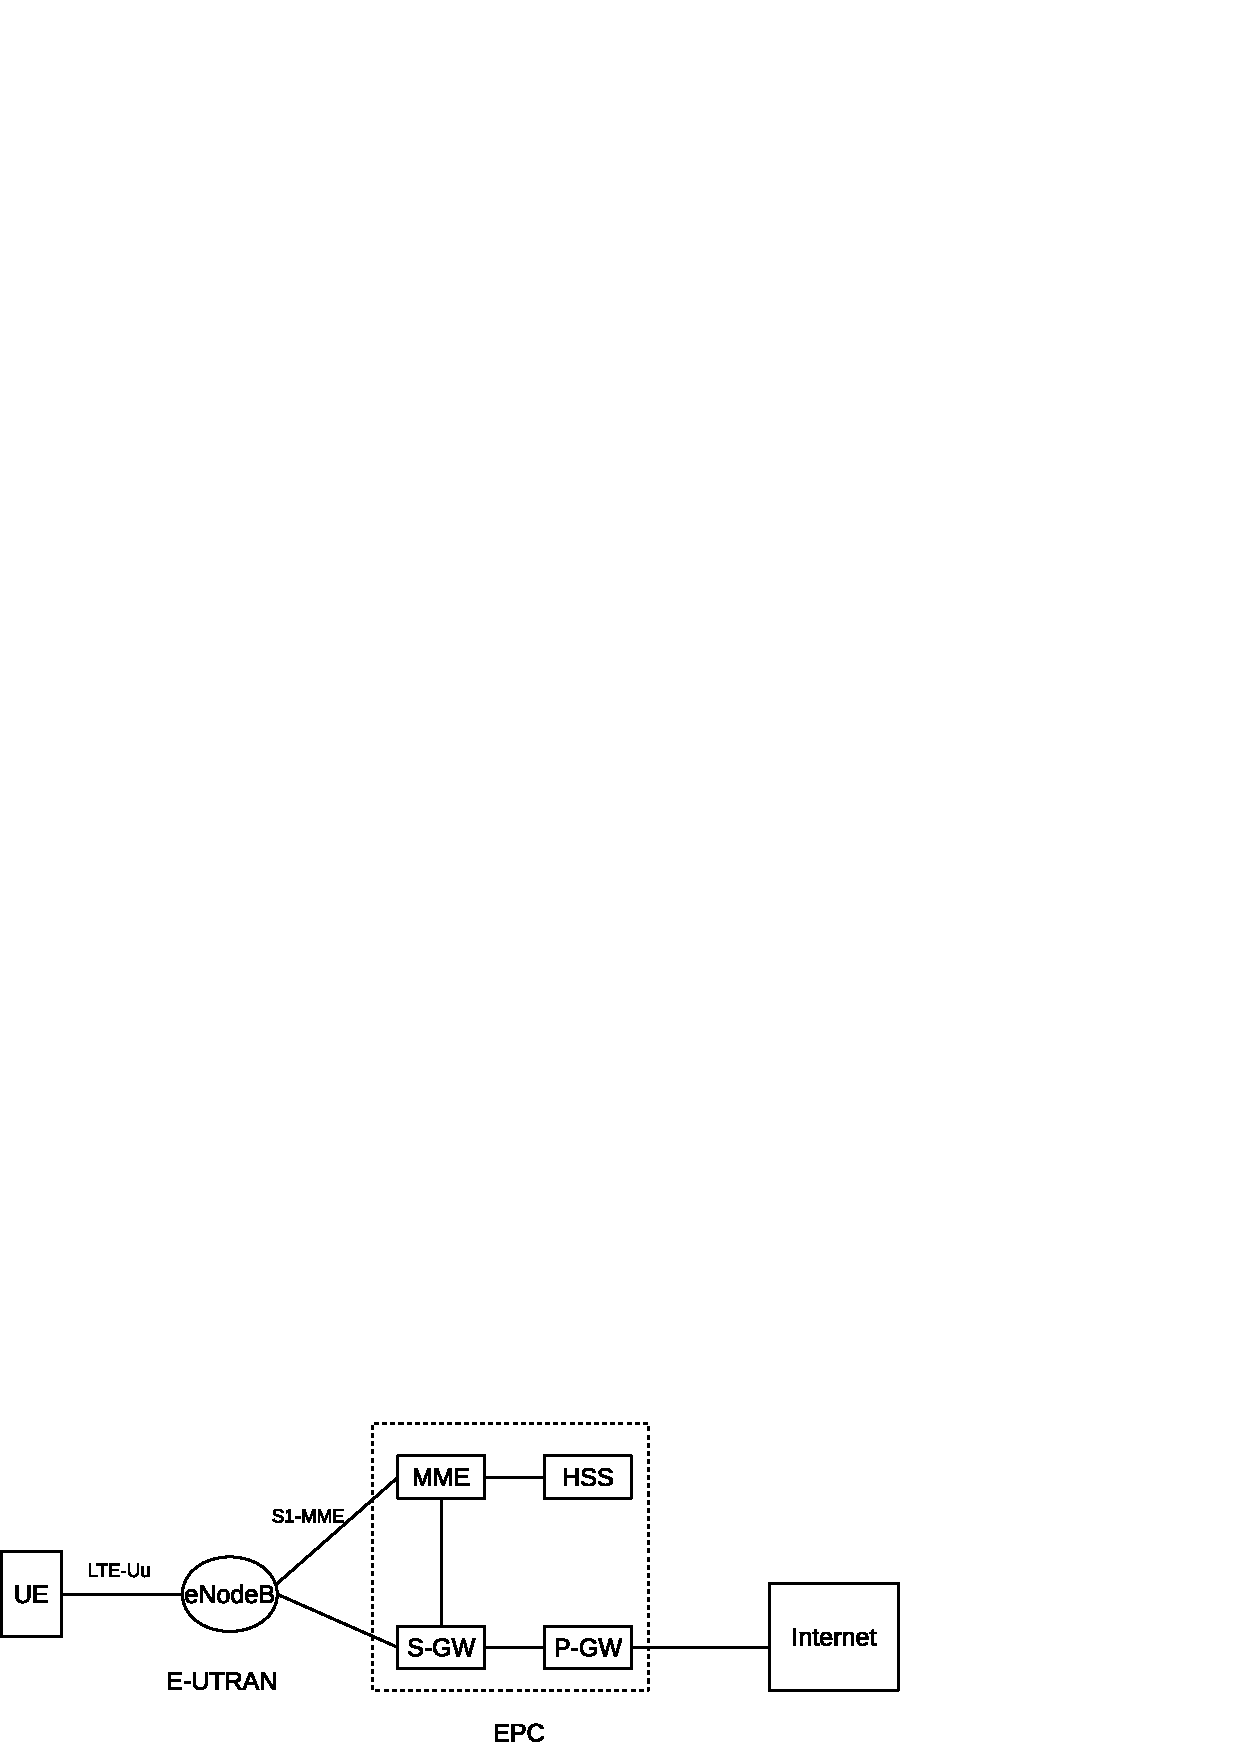
\includegraphics[width=0.45\textwidth]{lte_architecture.jpg}
% figure caption is below the figure
\caption{LTE Architecture, it is a dummy figure, I will draw my own figure}
\label{fig:protocl_stack}       % Give a unique label
\end{figure}

The UE is connected to the network via a radio link only with the radio network. The entity of the E-UTRAN that has the radio link with the UE is called eNodeB which is tradionally known as a base station. However, the UE also establishes a direct logical connection with an entity of the core network known as mobility management entity (MME). This logical connection is used only for the control signals for the core network and hence we do not focus on it in this paper. The user data as mentioned in the introduction travels from the UE to the eNodeB. Figure \ref{fig:protocl_stack} shows the protocol stack that the data travel across at the UE and at eNodeB. The L1 layer is the physical layer. We logically bundle the PDCP,RLC and MAC layers as layer 2 (L2) layer. All the encryption and decryption takes place at the PDCP layer \textcolor{red}{(cite)}

\begin{figure}
% Use the relevant command to insert your figure file.
% For example, with the graphicx package use
  \includegraphics[width=0.50\textwidth]{protocl_stack.png}
% figure caption is below the figure
\caption{Protocol stack, it is a dummy figure, I will draw my own figure}
\label{fig:protocl_stack}       % Give a unique label
\end{figure}

According to %\cite{EEA1_EEA2}, 
there are two encryption schemes in the 4th generation cellular network (LTE) developed by 3GPP. One is EEA1 in which the stream cipher SNOW 3G is used. The other is EEA2 in which the block cipher AES is used. The aspiration about 5G networks is to obtain at least 1Gbps data-rate. The question arises, if there are implementations of these two encryption systems that can achieve the required throughput and still be enough energy efficient to use in a mobile phone.

\section{Throughput and energy requirements of AES and SNOW 3G}
\label{sec:throughput_and_energy_requirements_of_aes_snow3g}
In \cite{IIS_Ruhr_2009}, the authors in their experiment showed that the computing power of a single embedded processor at reasonable clock frequencies is not enough to cope with the L2 requirements of LTE and next generation mobile devices. They illustrated that a conventional hardware acceleration approach for the encryption algorithms fail to offer the performance required by LTE and future mobile devices. The AES decryption was identified as the major time critical software algorithm, demanding half of the entire L2 DL execution time.


In a study in 
%\cite{IIS_Ruhr_2010}
 conducted in 2010 on the L2 DL layer (MAC,PDCP,RLC) layer, it has has been shown that by an sDMA, the authors did not mention anything about the achieved throughput but said that, it is enough for an LTE terminal. However, to achive this required throughput, the implementation consumed 9.5 mW of power whereas AES and SNOW 3G each required .5 and .57 mW of power respectively. Which means the encryption/decryption consumes around 5 percent of the power budget of L2 DL. (see in figure 6)AES

Whereas, a very recent study done in 2014, presented in 
%\cite{KTH_2014},
conducted on the UDP/IP layer, shows that (in Table II) an ASIC implementation consumes $14.62$ nano Joule of energy for a Kilobyte data in this layer. Which means it takes $(14.62/8)*1000 = 1827$ micro Joule of energy for 1 Giga bit data while providing throughtput of 2.24 Gbps..

Researchers have focused on implementing these cryptosystems both in hardware and software to achieve the required throughput. Looking up in the existing literature, it has been found that there exists implementations of these two cryptosystems that can achieve the required throughput even for a 5G network, that is at least 1 Gbps. However, there is no concrete account available of the power consumption of these implementations that enables the readers to estimate the energy share of the task of encryption across the entire protocol stack.

We have studied, collected and rendered the relevant information available in the literature into this single article in an easily comprehensible and comparable manner and make a case that the energy share of data encryption is too low to think of any alternative lightweight encryption for 5G enabled mobile phone.



\section{Overall comparison}
\label{sec:overall_comparison}

\section{Encryption is time consuming}
\label{sec:encryption_is_time_consuming}







\section{AES}
\label{sec:aes}

Since the adoption of Rijndael as AES by NIST, there have been number of hardware implementations of AES to achieve efficiency and high throughput. The below table gives a picture \newline


%\begin{tabular}{ |p{1cm}|p{.7cm}|p{.5cm}|p{1.2cm}|p{1cm}|p{1cm}|p{1cm}|p{1cm}|p{2cm}|p{1cm}|}
%\hline
%\multicolumn{10}{|c|}{AES Implementations} \\
%\hline
%Year &Tech &Ref &TP (Gbps) &Gates (K) & Clock Speed (MHz)&Power (mW) & Scal-able (Y/N) & Throughput per Kilo Gates in Gpbs & Energy per Gbit in $\mu$Joule \\ %\hline
%2001 & $.11 \mu$ & \cite{IBM_Japan_2001} &$2.6$ &$21.3$  & 0& - & Y & 0.122 & - \\ \hline
%2001 & $.11 \mu$ & \cite{IBM_Japan_2001} &$.311$ &$5.4$  & 0& - & Y & 0.0576 & - \\ \hline
%2001 & - & \cite{IBM_India_IIT_2001} &$.24$ &$4$  & 0& - & Y & 0.06 & - \\ \hline
%2006 & $.18 \mu$ & \cite{Taiwan_2006} &$.570$ & - & 48&20.34 &Y & - & 35684 \\ \hline
%2006 & $.35 \mu$ & \cite{Taiwan_2006} &$.569$ & - & 48&192.5 &Y & - & 338312 \\ \hline
%2007 & $.18 \mu$ & \cite{IIT_Kharagpur_2007} &$.384$ &$21$ & 120&- &Y & 0.018 & - \\ \hline
%2009 & $.18 \mu$ & \cite{IME_China_Tsinghua_Univerisity_2009} &$1.16$ &$19.47$ & - & - &Y & 0.056 & - \\ \hline
%2009 & $.09 \mu$ & \cite{Ruhr_2009} &$1.86$ &$15.25$ & 450&.78 &Y & 0.015 & 419 \\ \hline
%2011 & $ - $ & \cite{Ruhr_2011} &$.114$ &$ - $ & 300&.02 &Y & -  & 186.18 \\ \hline
%2012 & $.18 \mu$ & \cite{Pune_2012} &$1.6$ &$58.445$ & 125&22.85 &Y & - & 14281 \\ \hline
%\end{tabular}



So far the best power figure is found in %\cite{Ruhr_2009}. The implementation is scalable. Interestingly the power figure doesn't increase linearly with the number of AES engines used. Let us assume that the required data rate in 5G is 1 Gbps. So, the timing requirement is: 7.45 nano seconds per byte. 


According to figure 9 in %\cite{Ruhr_2011}, it will take roughly $.02*5=.1 mW$ for 1Gbps throughput. Because SAME has throughput of 114Mbps. And it achieves $5.5Mbps/ \mu J$. Which means it spends $114/5.5 = 20.72\mu J = .02 mW$. Now, by scaling up by 10 times, it will spend $.02*10=.2mW$ to achieve 1.14Gbps throughput


Comparing the best figure from the above table with %\cite{KTH_2014}, we see that ciphering takes $186/1827=.1$ or 10 percent energy of data communication on a ASIC packet processor.


In the study in %\cite{IIS_Ruhr_2010}, it was found that encryption was taking 5 or 6 percent of the power budget. However, as because other aspects of the protocol stack could be made more efficient, the power budget of encryption/decryption has increased.

So, with the current best implementation of the encryptor/decryptor hardware engine, in near future the power budget will only increase. However, now we need to check if 10 percent of the power budget for encryption will be good enough for a 5G phone or not.

%\begin{acknowledgements}
%If you'd like to thank anyone, place your comments here
%and remove the percent signs.
%\end{acknowledgements}

% BibTeX users please use one of
\bibliographystyle{spbasic}      % basic style, author-year citations
%\bibliographystyle{spmpsci}      % mathematics and physical sciences
%\bibliographystyle{spphys}       % APS-like style for physics
\bibliography{sources}   % name your BibTeX data base


\end{document}
% end of file template.tex
